\chapter{Concept Skteches}\label{cp:concept_sketches}

\section{Variant 1 - Original Design}

Concept sketch variant one, shown in \autoref{fig:sketch_01}, is our favorite design for our \acrshort{uav}. It is the simplest of the three designs and follows a common design pattern we noted from \acrshort{cots} \acrshort{rc} aircraft and past senior design projects.

\begin{figure}[htpb]
    \centering
    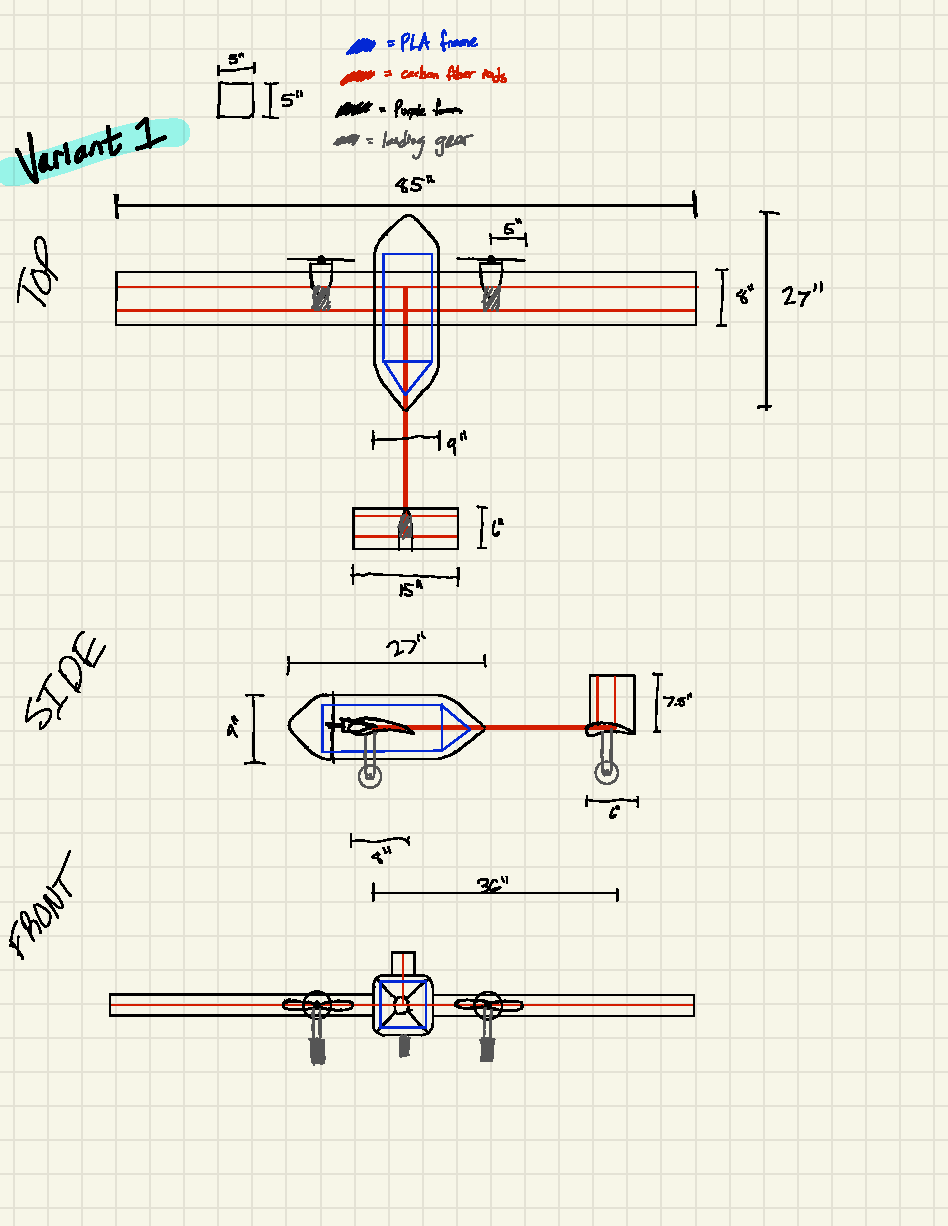
\includegraphics[width=0.7\linewidth]{Figures/aircraft_sketch_01.pdf}
    \caption[Concept sketch variant 1]{}
    \label{fig:sketch_01}
\end{figure}

\newpage

\section{Variant 2 - Wider and Flatter Fuselage}

Variant two, shown in \autoref{fig:sketch_02}, features a wider and flatter to reduce drag and weight. This design would be dependent on the smaller fuselage still being able to hold the Banshee's required payload, batteries, and electronics.

\begin{figure}[htpb]
    \centering
    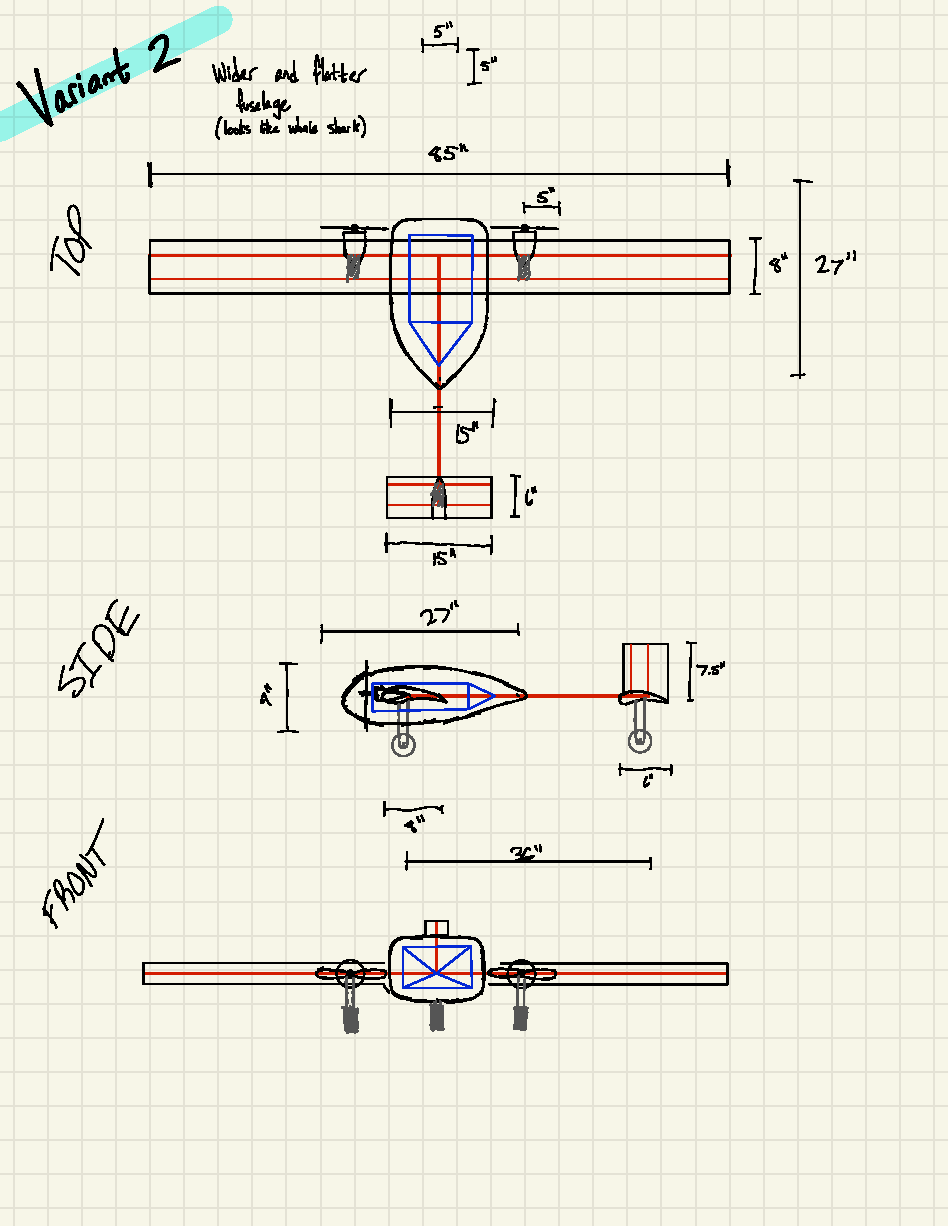
\includegraphics[width=0.9\linewidth]{Figures/aircraft_sketch_02.pdf}
    \caption[Concept sketch variant 2]{}
    \label{fig:sketch_02}
\end{figure}

\newpage

\section{Variant 3 - Wing-Integrated Fuselage}

The final variant, shown in \autoref{fig:sketch_03}, is more unconventional and may be harder to manufacture and structurally analyze. It features a wing-integrated fuselage, which—besides looking cool—may significantly reduce drag.

\begin{figure}[htpb]
    \centering
    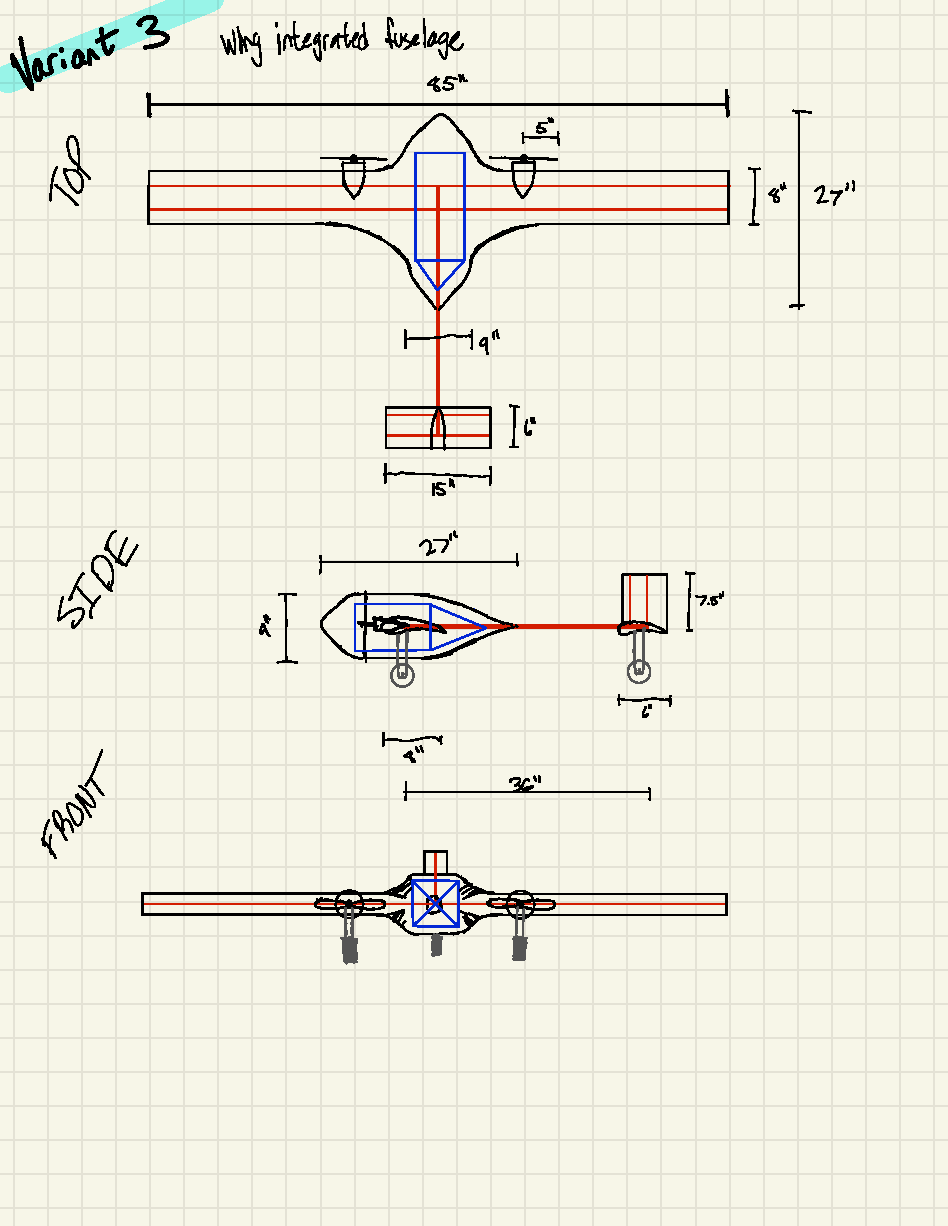
\includegraphics[width=0.9\linewidth]{Figures/aircraft_sketch_03.pdf}
    \caption[Concept sketch variant 3]{}
    \label{fig:sketch_03}
\end{figure}
